\subchapter{Lab1: Building and Booting a Preempt-RT Kernel}{Download, Configure, Build and Boot}

During this lab, you will:
\begin{itemize}

  \item Configure the project and choose a target
  \item Build your first Poky image
\end{itemize}

\section{Initial Setup}
As specified in the Buildroot
manual\footnote{\url{https://buildroot.org/downloads/manual/manual.html\#requirement-mandatory}},
Buildroot requires a few packages to be installed on your
machine. Let's install them using Ubuntu's package manager:

\begin{bashinput}
sudo apt install sed make binutils gcc g++ bash patch \
  gzip bzip2 perl tar cpio python unzip rsync wget libncurses-dev
\end{bashinput}

\section{Download Buildroot}

Since we're going to do Buildroot development, let's clone the
Buildroot source code from its Git repository:

\begin{bashinput}
git clone https://git.buildroot.net/git/buildroot.git
\end{bashinput}

In case this is blocked on your network, you can download the Buildroot
tarball \code{buildroot-2021.02.tar.bz2} from
\code{https://buildroot.org/downloads/} and extract it. However in this
case, you won't be able to use {\em Git} to visualize your changes and
keep track of them.

Go into the newly created \code{buildroot} directory.

We're going to start a branch from the {\em 2021.02} Buildroot
release, with which this training has been tested.

\begin{bashinput}
git checkout -b felabs 2021.02
\end{bashinput}

\section{Configuring Buildroot}

If you look under \code{configs/}, you will see that there is a file
named \code{beaglebone_defconfig}, which is a ready-to-use Buildroot
configuration file to build a system for the BeagleBone Black Wireless
platform.

We'll use that configuration as a basis for our setup :

\begin{bashinput}
make beaglebone_defconfig
\end{bashinput}

We'll configure Buildroot to download the Linux Kernel with the RT Patch applied.

From the \code{make menuconfig} interface, change the Kernel sources's custom
tarball location to the following :

\code{$(call github,beagleboard,linux,5.10.30-ti-rt-r3)/linux-5.10.30-ti-rt-r3.tar.gz}

Make sure you enable a toolchain with wchar and C++ support, it will be required
for later.

Realtime applications should really be using the GLibC, so select this C library in the
toolchain configuration.

\section{Kernel configuration}

Let's modify our kernel configuration to enable some required options :

\begin{bashinput}
	make linux-menuconfig
\end{bashinput}

Add the below options to support networking over USB device:
\begin{itemize}
  \item \kconfigval{CONFIG_USB_GADGET}{y}
  \item \kconfigval{CONFIG_USB_MUSB_HDRC}{y} {\em Driver for the USB OTG
        controller}
  \item \kconfigval{CONFIG_USB_MUSB_GADGET}{y} {\em Use the USB OTG controller
	in device (gadget) mode}
  \item \kconfigval{CONFIG_USB_MUSB_DSPS}{y}
  \item Check the dependencies of \kconfig{CONFIG_AM335X_PHY_USB}
        and find the way to set \kconfigval{CONFIG_AM335X_PHY_USB}{y}
  \item Find the "USB Gadget precomposed configurations" menu
        and set it to {\em static} instead of {\em module}
	so that \kconfigval{CONFIG_USB_ETH}{y}
\end{itemize}

Finally, make sure to select the right preemption model, and let's build our image !

\begin{bashinput}
make
\end{bashinput}

While the build is ongoing, don't hesitate to take a look at the latest
version of the patchset :

\begin{bashinput}
wget https://cdn.kernel.org/pub/linux/kernel/projects/rt/5.14/patches-5.14.1-rt19.tar.gz
\end{bashinput}

Look at the \code{series} file for more information about each individual patch.

\section{Setting up serial communication with the board}

The Beaglebone serial connector is exported on the 6 pins close to one
of he 48 pins headers. Using your special USB to Serial adapter provided
by your instructor, connect the ground wire (blue) to the pin closest
to the power supply connector (let's call it pin 1), and the \code{TX} (red)
and \code{RX} (green) wires to the pins 4 (board \code{RX}) and
5 (board \code{TX})\footnote{See
\url{https://www.olimex.com/Products/Components/Cables/USB-Serial-Cable/USB-Serial-Cable-F/}
for details about the USB to Serial adapter that we are using.}.

You always should make sure that you connect the \code{TX} pin of the cable
to the \code{RX} pin of the board, and vice-versa, whatever the board and
cables that you use.

\begin{center}
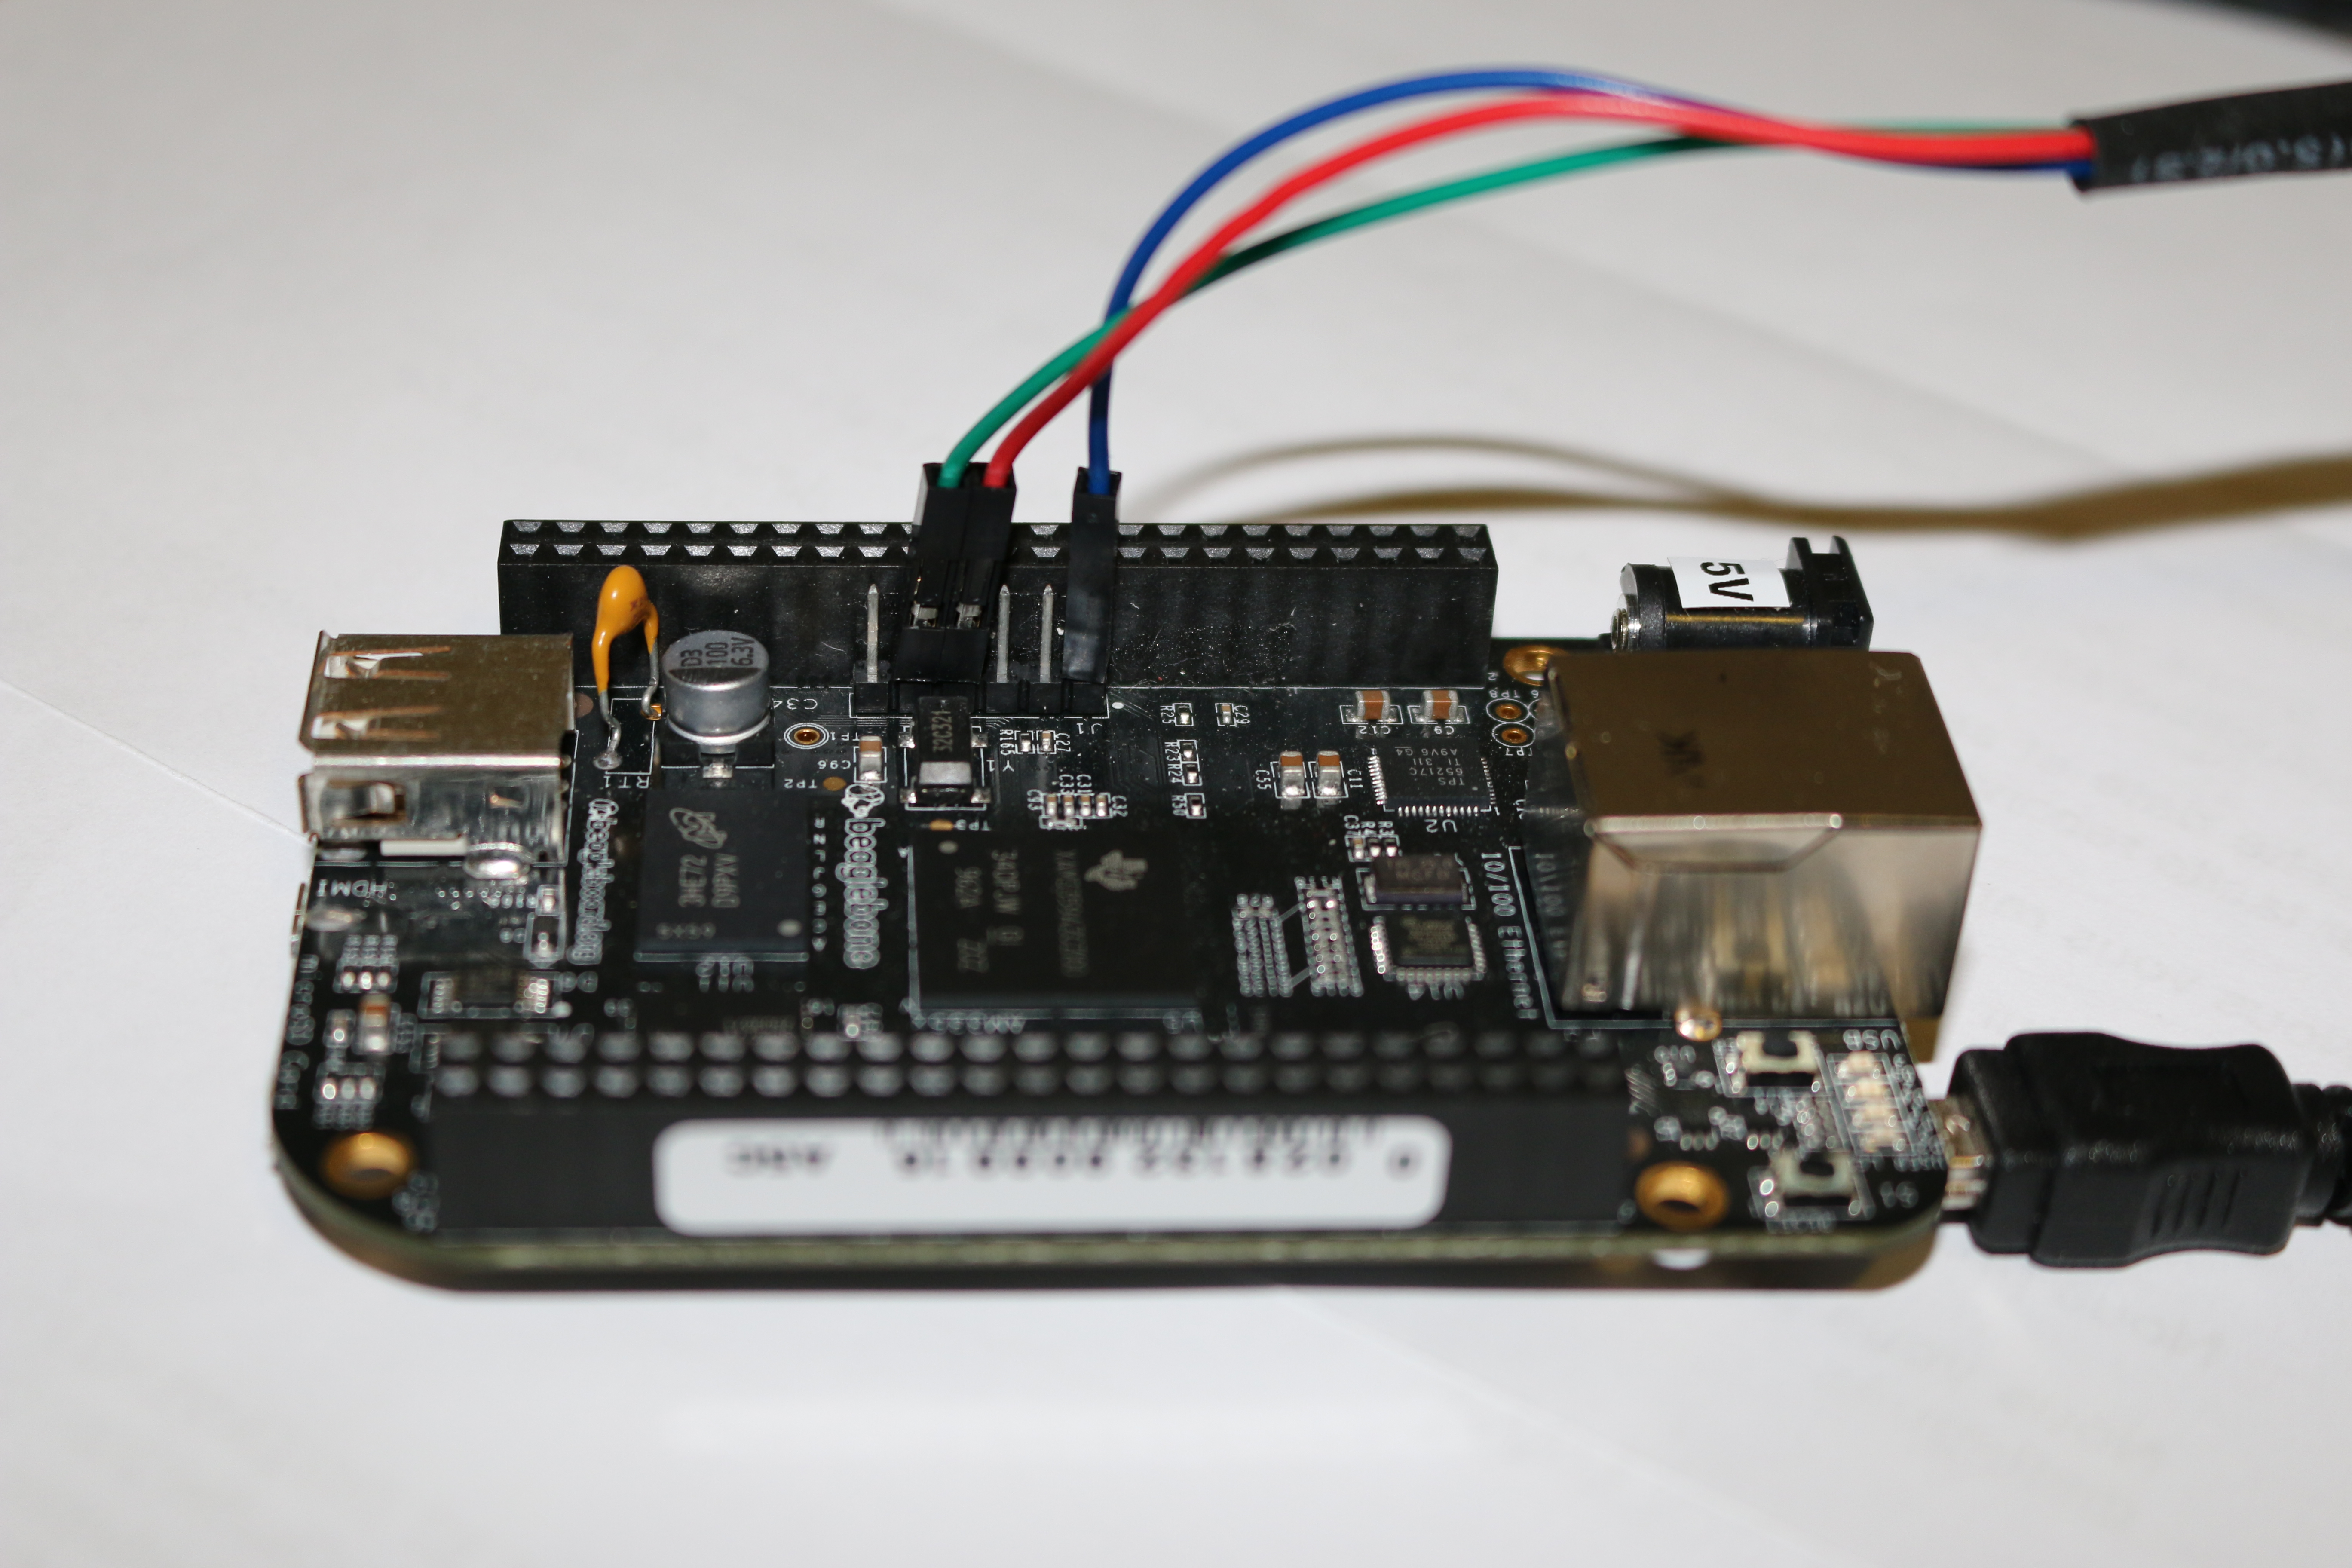
\includegraphics[width=8cm]{common/beaglebone-black-serial-connection.jpg}
\end{center}

Once the USB to Serial connector is plugged in, a new serial port
should appear: \code{/dev/ttyUSB0}.  You can also see this device
appear by looking at the output of \code{dmesg}.

To communicate with the board through the serial port, install a
serial communication program, such as \code{picocom}:

\begin{bashinput}
sudo apt install picocom
\end{bashinput}

If you run \code{ls -l /dev/ttyUSB0}, you can also see that only
\code{root} and users belonging to the \code{dialout} group have
read and write access to this file. Therefore, you need to add your user
to the \code{dialout} group:

\begin{bashinput}
sudo adduser $USER dialout
\end{bashinput}

{\bf Important}: for the group change to be effective, in Ubuntu 18.04, you have to
{\em completely reboot} the system \footnote{As explained on
\url{https://askubuntu.com/questions/1045993/after-adding-a-group-logoutlogin-is-not-enough-in-18-04/}.}.
A workaround is to run \code{newgrp dialout}, but it is not global.
You have to run it in each terminal.

Now, you can run \code{picocom -b 115200 /dev/ttyUSB0}, to start serial
communication on \code{/dev/ttyUSB0}, with a baudrate of \code{115200}. If
you wish to exit \code{picocom}, press \code{[Ctrl][a]} followed by
\code{[Ctrl][x]}.

There should be nothing on the serial line so far, as the board is not
powered up yet.

\section{Configure the U-Boot environment and boot}

Flash the generated image onto your SD card :

\begin{bashinput}
	sudo dd if=output/images/sdcard.img of=/dev/mmcblk0 bs=1M conv=fdatasync
\end{bashinput}


Insert the SD card in the dedicated slot on the BeagleBone Black. Press the S2
push button (located just above the previous slot), plug in the USB cable and
release the push button.

Enter the U-boot prompt, and change the boot environment variables with the following commands :

\begin{bashinput}
setenv bootcmd 'mmc rescan; fatload mmc 0 0x80200000 zImage; fatload mmc 0 0x82000000 am335x-boneblack.dtb; bootz 0x80200000 - 0x82000000'
setenv bootargs 'console=ttyS0,115200 root=/dev/mmcblk0p2 rootwait rw'
saveenv
\end{bashinput}

Wait until the login prompt, then enter \code{root} as user.
Congratulations! The board has booted and you now have a shell.

